\documentclass{beamer}

\usepackage[utf8]{inputenc}
\usepackage[T1]{fontenc}
\usepackage{graphicx}
\usepackage{lmodern}
\usepackage{textpos}
\usepackage{pgf-umlsd}
\usepackage{listings}
\usepackage{tikz}
\usepackage{pgfplots}
\usepackage{pgfplotstable}
\usepackage[numbers,sort&compress]{natbib}
\usepackage{graphicx}
\usepackage{subcaption}

\usepgfplotslibrary{statistics}


\usepackage{t1enc}
\usepackage[utf8]{inputenc}
\usepackage{lmodern}

\usepackage[title,titletoc]{appendix}
\usepackage[section]{placeins}
\usepackage{relsize}

\usepackage[normalem]{ulem} %% Provides underlining.
\usepackage{caption} %% Provides captions.
\usepackage{mdframed} %% Provides frames around text and equations.
\usepackage{tikz-cd} %% Provides diagram drawing environment.
\usepackage{adjustbox} %% Provides additional tools to resize content.
% \usepackage[magyar]{babel} %% Provides foreign language support.

%%%%
%% Provides math related environments and directives.
\usepackage{amssymb}
\usepackage{amsthm}
\usepackage{amsmath}
\usepackage{latexsym}

\usepackage{dsfont}
\usepackage{commath}
\usepackage{bm}
\usepackage{subcaption}

%% See http://tex.stackexchange.com/questions/43835/conflict-between-amsthm-and-some-other-package
\let\proof\relax 
\let\endproof\relax

%%%%
%% Provides table environments and related directives.
\usepackage{array}
\usepackage{tabulary}
\usepackage{tabularx}
\usepackage{multirow}
\usepackage{hhline}
\usepackage{diagbox}
\usepackage{array}

%%%%
%% Provides figure environments and related directives.
\usepackage{graphicx}
\makeatletter
\def\maxwidth#1{\ifdim\Gin@nat@width>#1 #1\else\Gin@nat@width\fi}
\def\maxheight#1{\ifdim\Gin@nat@height>#1 #1\else\Gin@nat@height\fi}
\makeatother

\usepackage{fancyvrb}
\usepackage{rotating}
\frenchspacing



% Fordításhoz: pdflatex

\newcommand{\N}{\mathbb{N}}
\newcommand{\Z}{\mathbb{Z}}
\newcommand{\R}{\mathbb{R}}
\newcommand{\C}{\mathbb{C}}
\newcommand{\Hq}{\mathbb{H}}
\newcommand{\D}{\mathbb{D}}

\newcommand{\qi}{\textbf{i}}
\newcommand{\qj}{\textbf{j}}
\newcommand{\qk}{\textbf{k}}
\newcommand{\qmu}{\boldsymbol{\mu}}

\DeclareMathOperator{\rp}{Re}
\DeclareMathOperator{\ip}{Im}

\def\n{n\in\N}
\def\x{x\in\R}
\def\N{{\mathbb N}}
\def\R{{\mathbb R}}
\def\C{{\mathbb C}}
\def\Z{{\mathbb Z}}
\def\D{{\mathbb D}}
\def\B{{\mathfrak B}}
\def\T{{\mathbb T}}
\def\btheta{{\boldsymbol{\vartheta}}}
\def\bgamma{{\boldsymbol{\gamma}}}
\def\bl{{\mathbf{l}}}
\def\bk{{\mathbf{k}}}
\def\bt{{\mathbf{t}}}
\def\be{{\mathbf{e}}}


\newtheorem{definicio}{Definíció}
\newtheorem{allitas}{Állítás}
\newtheorem{kov}{Következmény}
\newtheorem{pelda}{Példa}
\newtheorem{tetel}{Tétel}


\usebackgroundtemplate{%

\includegraphics[width=\paperwidth,height=\paperheight]{background.jpg}%
}

%\setbeamercolor{title}{fg=white}
%\setbeamercolor{author}{fg=white}
%\setbeamercolor{institute}{fg=white}
%\setbeamercolor{date}{fg=white}
\setbeamercolor{frametitle}{fg=white}
%
%\title{\bf Presentation heading}
%\author{Sample Samuel}
%\institute{Eötvös Loránd University (ELTE), Budapest, Hungary}
%\date{2018}

\pgfplotsset{compat=1.16}

\begin{document}

{
\usebackgroundtemplate{
\includegraphics[width=\paperwidth]{title.jpg}}%
\begin{frame}

\color{white}{

\textbf{\Large{Színes képek elemzése és felismerése kvaternió Zernike momentumok segítségével}}
% \textbf{\Large{Color image analysis and recognition using quaternion Zernike moments}}

\bigskip

\Large{Nagy Gergely}

\bigskip

\footnotesize{Eötvös Loránd Tudományegyetem, Informatikai Kar}
\bigskip


\large{Tudományos Diákköri Konferencia}\\
\footnotesize{Budapest, 2020. május 28.}
\vspace{2em}

% Szakmai beszámolókhoz: (Igazi neveket kérünk feltüntetni.) Más előadáson nem kell.
\begin{footnotesize}
Témavezető: Németh Zsolt
\end{footnotesize}
\bigskip

% pozícionáljuk a dia aljához közel
\begin{textblock}{8}(0,2.5)
\footnotesize{EFOP-3.6.3-VEKOP-16-2017-00001}
\end{textblock}
}


\end{frame}
}

% \begin{frame}
%     \frametitle{Tartalom}
%     \tableofcontents
% \end{frame}

\section{Háttér}
\subsection{Momentumok}
\begin{frame}{Momentumok}
Általában valamilyen leíró érték a pixel intenzitások alapján, 
például geometriai momentumok: $$M_{ij} = \sum_x\sum_y x^i y^j I(x,y).$$
\textbf{Zernike momentumok}: az egységkörön definiált, ortogonális Zernike függvények alapján
$$Z_{n,m}(f) = \frac{n+1}{\pi}\int_0^1\int_0^{2\pi}f(r,\theta)R_{n,m}(r)e^{-\qi m\theta} dr d\theta,$$ ahol $R_{n,m}(r)$ az ortogonális, sugárirányú polinomok.\\

\textbf{Momentumok invariánsok:} forgatás, skálázás és eltolás invariancia 
\end{frame}

\subsection{Színes képek}
\begin{frame}{Momentumok alkalmazása színes képekre}
Hagyományos megoldások:
\begin{itemize}
    \item A kép szürkeárnyalatossá alakítása.
    \item Külön-külön a színcsatornákra.
\end{itemize}
Utóbbi évtizedben:\\
$f : \R^2 \rightarrow \R^3$ kép kvaternió értékű függvényként:
$$f(x,y) = \qi f_R(x,y) + \qj f_G(x,y) + \qk f_B(x,y)$$
Különböző momentumok általánosítása kvaterniókra:\\
QFMM (Fourier-Mellin), QG-CHFM (Csebisev-Fourier), QG-PJFM (Jacobi-Fourier), QBFM (Bessel-Fourier), \\
\textbf{QZM (Zernike)}
\end{frame}

\begin{frame}{Kvaternió Zernike momentumok}
\vskip 3mm
Zernike függvények általánosítása kvaterniókra: $$\Phi_{n,m}(r,\theta) = R_{n,m}(r)e^{-\qmu m \theta},$$ ahol $\qmu$ egység hosszú, tiszta kvaternió (általában $\qmu = \frac{\qi + \qj + \qk}{\sqrt{3}}$).

Mivel a kvaterniók szorzása nem kommutatív, így jobb- és baloldali momentumok is definiálhatók:
$$Z^R_{n,m}(f) = \frac{n+1}{\pi}\int_0^1\int_0^{2\pi}f(r,\theta)\Phi_{n,m}(r,\theta) dr d\theta,$$
$$Z^L_{n,m}(f) = \frac{n+1}{\pi}\int_0^1\int_0^{2\pi}\Phi_{n,m}(r,\theta)f(r,\theta) dr d\theta.$$

Chen et al.: forgatás, skálázás és eltolás kombinált invariánsok ($\overline{\Psi}_{n,k}^m$) konstruálása.
\end{frame}

\section{Diszkretizáció}
\subsection{Korábbi módszer}
\begin{frame}{Korábbi diszkretizációs módszer}
    \vskip 5mm
    \begin{figure}[tb]
        \begin{subfigure}{.30\textwidth}
        \centering
          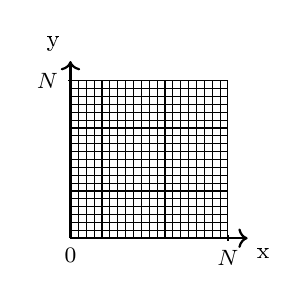
\begin{tikzpicture}
            \draw[step=0.1cm,black] (0,0) grid (2,2);
            \draw[thick,->] (0,0) -- (2.25,0) node[anchor=north west] {\footnotesize x};
            \draw[thick,->] (0,0) -- (0,2.25) node[anchor=south east] {\footnotesize y};
            \draw (2cm,1pt) -- (2cm,-1pt) node[anchor=north] {\footnotesize$N$};
            \draw (1pt,2cm) -- (-1pt,2cm) node[anchor=east] {\footnotesize$N$};
            \draw (0,0) -- (0,0) node[anchor=north] {\footnotesize$0$};
          \end{tikzpicture}
        \end{subfigure}
        \begin{subfigure}{.05\textwidth}
          \centering
          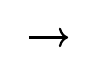
\begin{tikzpicture}
            \draw[thick,->] (0,0) -- (0.5,0);
          \end{tikzpicture}
        \end{subfigure}
        \begin{subfigure}{.30\textwidth}
          \centering
            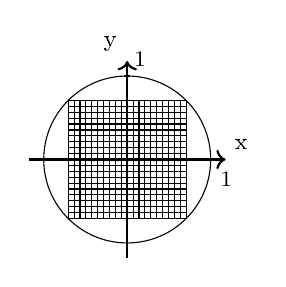
\begin{tikzpicture}
              \draw[step=0.075cm,black] (-0.75,-0.75) grid (0.75,0.75);
              \draw[thick,->] (-1.25,0) -- (1.25,0) node[anchor=south west] {\footnotesize x};
              \draw[thick,->] (0,-1.25) -- (0,1.25) node[anchor=south east] {\footnotesize y};
              \draw (0,0) circle (1.06cm);
              \draw (1.06cm,1pt) -- (1.06cm,-1pt) node[anchor=north west] {\footnotesize $1$};
              \draw (1pt,1.06cm) -- (-1pt,1.06cm) node[anchor=south west] {\footnotesize $1$};
            \end{tikzpicture}
          \end{subfigure}
      \end{figure}
      \begin{itemize}
          \item Kép transzformálása az egységkörbe: \\
                $r_{x,y} = \sqrt{(c_1x + c_2)^2 + (c_1y + c_2)^2},\ \ \ \  \theta_{x,y} = \tan^{-1}\left(\frac{c_1y + c_2}{c_1x + c_2}\right),$\\
                ahol $c_1 = \frac{\sqrt{2}}{N-1}$ és $c_2 = -\frac{1}{\sqrt{2}}$.
          \item Ekkor a pixelek helyét alappontoknak választva:\\
                $$Z^R_{n,m}(f) \approx \frac{2(n+1)}{\pi(N-1)^2}\sum_{x=0}^{N-1}\sum_{y=0}^{N-1}f(x,y)\Phi_{n,m}(r_{x,y},\theta_{x,y}).$$
      \end{itemize}
\end{frame}

\subsection{Új módszer}
\begin{frame}{Új diszkretizációs módszer}
    Probléma a korábbi diszkretizációval: nincs diszkrét ortogonalitás.
    \vskip 5mm
    Schipp F. és Pap M.: diszkrét ortogonális pontrendszer konstrukciója a klasszikus (komplex értékű) Zernike függvényekhez.
    \vskip 3mm
    Ennek az ötletnek a kvaternió értékű Zernike függvényekre való kiterjesztése megfelelő pontrendszert ad.
    \vskip 3mm
    Legyen $N$ pozitív egész és $\rho_{k,N}$ az $N$-edik Legendre polinom gyökei, ekkor a pontrendszer:
    $$(r_{k,N}, \theta_{j,N}) = \left(\sqrt{\frac{1+\rho_{k,N}}{2}} , \frac{2\pi j}{4N} \right), \ (k=1,\ldots,N,j=1,\ldots,4N).$$
    
\end{frame}

\begin{frame}{Új diszkretizációs módszer (folyt.)}
    \vskip 5mm
    Legyen $$\mathcal{A}_{k,N} = \int_{-1}^{1} \ell_{k,N}(x)\ dx, \ (k=1,\ldots,N),$$ ahol $\ell_{k,N}$ a Lagrange interpolációs alappolinomok a $\rho_{k,N}$ pontokon.\\
    Ekkor a $w(r_{k,N},\theta_{j,N}) = \frac{\mathcal{A}_{k,N}}{8N}$ súlyokkal véve az integrálközelítést:
    $$\frac{1}{\pi} \int_{0}^1 \int_0^{2\pi} f(r,\theta)\ d\theta dr \approx \int_{X_N} f = \sum_{k=1}^{N} \sum_{j=1}^{4N} f(r_{k,N},\theta_{j,N}) \frac{\mathcal{A}_{k,N}}{8N}.$$
    Azaz a QZM-ek közelíthetők a következő módon:
    $$Z^R_{n,m}(f) \approx (n+1)\sum_{k=1}^{N}\sum_{j=1}^{4N}f(r_{k,N},\theta_{j,N})\Phi_{n,m}(r_{k,N},\theta_{j,N})\frac{\mathcal{A}_{k,N}}{8N}.$$

\end{frame}


\subsection{Diszkrét ortogonalitás}
\begin{frame}{Diszkrét ortogonalitás}
\begin{tetel}[Diszkrét ortogonalitás]
    Legyen $n, n' \in \N$ természetes számok, $m, m' \in \Z$ egészek, úgy, hogy teljesül $$\frac{n + n'}{2} + \min(|m|,|m'|) < 2N.$$
    Ekkor $$(n + 1)\int_{X_N}\Phi_{n,m}\Phi_{n',m'}^* = \delta_{n,n'}\delta_{m,m'}.$$
\end{tetel}
Így a momentumok diszkretizációs hiba nélkül előállíthatók és a képek visszaállítási pontossága és módszer hibatűrése is javult.
\end{frame}

\begin{frame}{Képpontok becslése}

\begin{columns}
    \begin{column}{0.5\textwidth}
        \begin{figure}
            \begin{subfigure}{.48\textwidth}
                \centering
            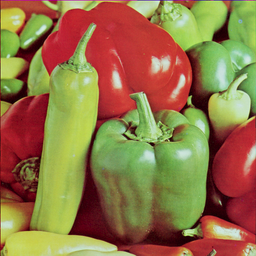
\includegraphics[width=\textwidth]{figures/pepper_color_256.png}
            \end{subfigure}
            \begin{subfigure}{.48\textwidth}
                \centering
            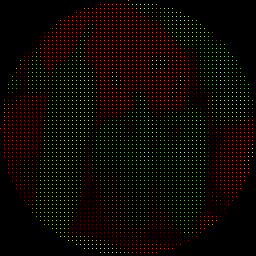
\includegraphics[width=\textwidth]{figures/pepper_square.png}
            \end{subfigure}
            \begin{subfigure}{.48\textwidth}
                \centering
            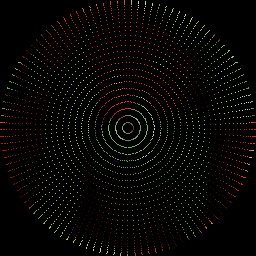
\includegraphics[width=\textwidth]{figures/pepper_bilinear.png}
            \end{subfigure}
            \begin{subfigure}{.48\textwidth}
                \centering
            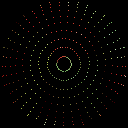
\includegraphics[width=\textwidth]{figures/pepper_integral.png}
            \end{subfigure}
        \end{figure}
    \end{column}
    \begin{column}{0.5\textwidth}
        A képet lineárisan transzformáljuk az egységkörre.
        \vskip 3mm
        A függvény értékének becslése a pontokban:
        \begin{itemize}
            \item Lineáris interpoláció (sok pont esetén)
            \item Diszkrét integrálás a pontok környezetében (kevés pont esetén)
        \end{itemize}
    \end{column}
\end{columns}

\end{frame}


\section{Eredmények}
\begin{frame}{Gyakorlati tesztek}
    \vskip 5mm
    A következő tesztek alapján hasonlítottuk össze a régi és az új módszert:
    \begin{itemize}
    \item Invariancia teszt
    \item Kép visszaállítása momentumokból
    \item Transzformált, zajos képek felismerése
    \end{itemize}
    A tesztek során a Columbia Object Image Library és az Amsterdam Library of Object Images képeiből generált transzformált képeket használtuk.
    \begin{figure}[tbp]
        \begin{subfigure}{0.3\textwidth}
            \centering
        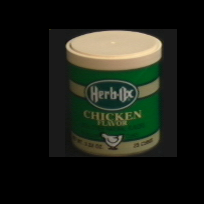
\includegraphics[width=70pt]{figures/coil_rst/26x-11y9r0s1_0.png}
        \end{subfigure}
        \begin{subfigure}{0.3\textwidth}
            \centering
        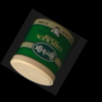
\includegraphics[width=70pt]{figures/coil_rst/26x-11y9r150s0_5.png}
        \end{subfigure}
        \begin{subfigure}{0.3\textwidth}
            \centering
        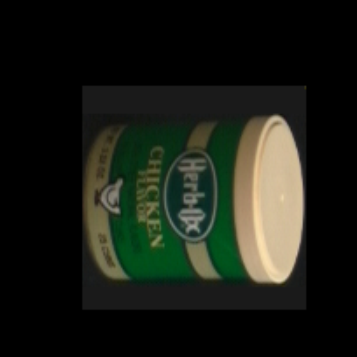
\includegraphics[width=70pt]{figures/coil_rst/26x-11y9r270s1_75.png}
        \end{subfigure}
    \end{figure}
\end{frame}

\subsection{Invariancia}
\begin{frame}{Invariancia}
    \vskip 10mm
Alacsony rendű momentumok modulusának, az összes transzformált képekre vett variációs koefficiense $\left(\frac{\sigma}{\mu}\right)$:
\begin{columns}
    \begin{column}{.5\textwidth}
        \begin{table}
            \centering
        \begin{tabular}{| c | c | } \hline
        & $\frac{\sigma}{\mu}$ \\ \hline\hline
        $|\overline{\Psi}_{1,1}^1|$ & 3.73\% \\ \hline
        $|\overline{\Psi}_{2,0}^0|$ & 0.028\% \\ \hline
        $|\overline{\Psi}_{2,2}^0|$ & 0.057\% \\ \hline
        $|\overline{\Psi}_{2,2}^2|$ & 6.87\% \\ \hline
        $|\overline{\Psi}_{3,1}^1|$ & 3.71\%  \\ \hline
        $|\overline{\Psi}_{3,3}^1|$ & 3.69\% \\ \hline
        $|\overline{\Psi}_{3,3}^3|$ & 9.40\% \\ \hline
        \end{tabular}
        \caption{Régi módszer}
        \end{table}
    \end{column}
    \begin{column}{.5\textwidth}
        \begin{table}
            \centering
        \begin{tabular}{| c | c | } \hline
        & $\frac{\sigma}{\mu}$ \\ \hline\hline
        $|\overline{\Psi}_{1,1}^1|$ & 3.72\% \\ \hline
        $|\overline{\Psi}_{2,0}^0|$ & 0.028\%\\ \hline
        $|\overline{\Psi}_{2,2}^0|$ & 0.056\%\\ \hline
        $|\overline{\Psi}_{2,2}^2|$ & 6.82\%\\ \hline
        $|\overline{\Psi}_{3,1}^1|$ & 3.70\%\\ \hline
        $|\overline{\Psi}_{3,3}^1|$ & 3.68\%\\ \hline
        $|\overline{\Psi}_{3,3}^3|$ & 9.32\%\\ \hline
        \end{tabular}
        \caption{Új módszer}
        \end{table}
    \end{column}
\end{columns}
\end{frame}

\newcolumntype{Q}{>{\centering\arraybackslash} m{13pt} }
\newcolumntype{q}{>{\centering\arraybackslash} m{42pt} }

\subsection{Rekonstrukció}
\begin{frame}{Képek visszaállítása}
\vskip 10mm
Egy kép rekonstruálható véges számú momentumot használva a következő képlet szerint:
$$
f(x,y) \approx \sum_{n=0}^{M}\sum_{m=-n}^{n}Z_{n,m}^R(f)\Phi_{n,m}^*(r_{x,y},\theta_{x,y}).
$$
Ha $f$ az eredeti, $\widehat{f}$ a visszaállított kép, akkor a hiba (mean square error):
\begin{gather*}
    \varepsilon^2 = \frac{\displaystyle \sum_{x=1}^N\sum_{y=1}^N \left|f(x,y) - \widehat{f}(x,y)\right|^2}{\displaystyle \sum_{x=1}^N\sum_{y=1}^N \left|f(x,y)\right|^2}.
\end{gather*}
\end{frame}

\begin{frame}{Képek visszaállítása}
    \begin{figure}
        \centering
    \begin{tabular}{c | q q q q q }
     & Eredeti & 50 & 100 & 150 & 250 \\ \hline\hline
    Régi & 
    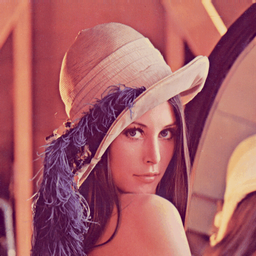
\includegraphics[width=50pt]{figures/reconstruction/lo256.png} &
    
\includegraphics[width=50pt]{figures/reconstruction/lo25650.png} &
    
\includegraphics[width=50pt]{figures/reconstruction/lo256100.png} &
    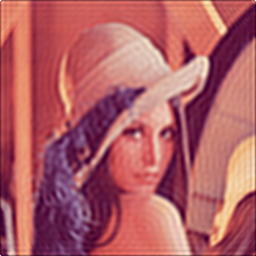
\includegraphics[width=50pt]{figures/reconstruction/lo256150.png} &
    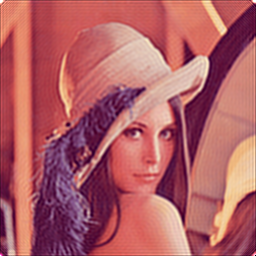
\includegraphics[width=50pt]{figures/reconstruction/lo256250.png} \\
    $\varepsilon^2$ & & 0.02659 & 0.1341 & 0.00868 & 0.00428 \\
    Új & 
    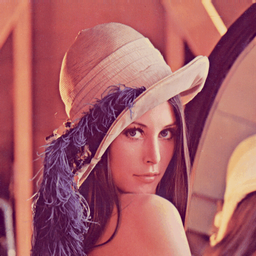
\includegraphics[width=50pt]{figures/reconstruction/lo256.png} &
    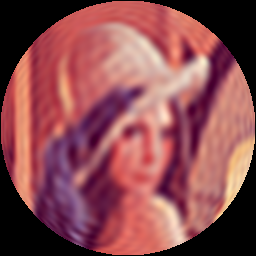
\includegraphics[width=50pt]{figures/reconstruction/ln25650.png} &
    
\includegraphics[width=50pt]{figures/reconstruction/ln256100.png} &
    
\includegraphics[width=50pt]{figures/reconstruction/ln256150.png} &
    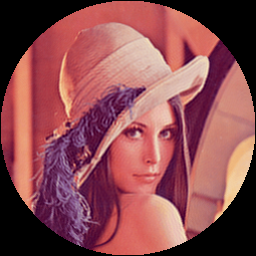
\includegraphics[width=50pt]{figures/reconstruction/ln256250.png} \\
    $\varepsilon^2$ & & 0.01611 & 0.00790 & 0.00463 & 0.00190  \\   
    \end{tabular}

    \end{figure}
\end{frame}

\subsection{Képfelismerés}
\begin{frame}{Képfelismerés}
    \vskip 5mm
Cél: a transzformált, zajos képet felismerni az eredeti képek közül.\\
Különböző nagyságú és típusú zaj:
\begin{itemize}
    \item Gauss zaj
    \item Só-bors zaj
\end{itemize}
Alacsony rendű invariáns momentumok (kvaterniók) komponenseiből kinyert valós értékek vektorként kezelése. Osztályozás legkisebb euklideszi távolság alapján.
\begin{figure}[tbp]
    \begin{subfigure}{0.25\textwidth}
        \centering
    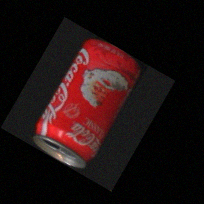
\includegraphics[width=\textwidth]{figures/noise/gauss5.png}
    \end{subfigure}
    \begin{subfigure}{0.25\textwidth}
        \centering
    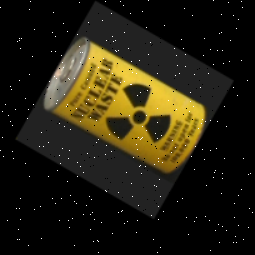
\includegraphics[width=\textwidth]{figures/noise/pepper1.png}
	\end{subfigure}
\end{figure}
\end{frame}

\begin{frame}{Képfelismerés - Gauss zaj}
    \vskip 1cm
    \begin{table}[tbp]
        \centering
        \begin{tabular}{|p{1.5cm}|p{1.5cm}|p{1.8cm}|p{2cm}|} \hline
            $\sigma$ & \textbf{Régi} (\%) & \textbf{Új} -- "sok" pont (\%)& \textbf{Új} -- "kevés" pont (\%) \\ \hline\hline
            Nincs zaj & 99.06 & 99.15 & 98.21 \\ \hline
            1 & 98.98 & 99.49 & 98.81 \\ \hline
            2 & 98.98 & 99.74 & 98.81 \\ \hline
            3 & 98.55 & 99.83 & 98.04 \\ \hline
            5 & 95.15 & 99.49 & 94.64 \\ \hline
            7 & 95.15 & 98.72 & 91.67 \\ \hline
            9 & 76.87 & 98.47 & 89.20 \\ \hline
            40 & 52.89 & 88.52 & 51.87 \\ \hline
            50 & 48.21 & 84.10 & 45.07 \\ \hline
            60 & 41.58 & 85.80 & 39.12 \\ \hline
        \end{tabular}
    \end{table}
\end{frame}

\begin{frame}{Képfelismerés - Só-bors zaj}
    \vskip 1cm
    \begin{table}[tbp]
        \centering
        \begin{tabular}{|p{1.5cm}|p{1.5cm}|p{1.8cm}|p{2cm}|} \hline
            p & \textbf{Régi} (\%) & \textbf{Új} -- "sok" pont (\%)& \textbf{Új} -- "kevés" pont (\%) \\ \hline\hline
            Nincs zaj & 99.06 & 99.15 & 98.21 \\ \hline
            0.2\% & 99.66 & 99.32 & 94.98 \\ \hline
            0.4\% & 99.91 & 99.74 & 99.15 \\ \hline
            0.6\% & 99.91 & 99.91 & 99.40 \\ \hline
            1\% & 98.98 & 99.91 & 99.66 \\ \hline
            2\% & 99.66 & 93.96 & 99.74 \\ \hline
            3\% & 99.40 & 99.40 & 96.34 \\ \hline
            5\% & 97.87 & 94.90 & 97.87 \\ \hline
            10\% & 99.91 & 93.03 & 98.72 \\ \hline
            15\% & 99.91 & 93.20 & 97.87 \\ \hline
        \end{tabular}
    \end{table}
\end{frame}

\section{Alkalmazások}
\begin{frame}{Alkalmazások}
    A momentumok sok területen alkalmazhatók, néhány példa:
    \begin{itemize}
    \item \textbf{Vízjelek}: a képre a momentumok szintjén helyeznek vízjelet, így ellenálló lesz különböző transzformációknak és zajnak. Ehhez fontos a rekonstrukciós pontosság.
    \item \textbf{Neurális hálók, gépi tanulás}: A képekből kinyert invariáns momentumok lehet a bemeneti vektor része. A neurális hálók ismert hiányossága a zajra való érzékenység, ezen segíthetnek a momentumok.
    \item \textbf{Orvosi/optikai alkalmazások}: lencsék leképezési hibáinak azonosítására, szaruhártya vizsgálatára, stb.
    \end{itemize}
\end{frame}

\begin{frame}{További lehetőségek}
    \begin{itemize}
    \item Meglévő alkalmazások továbbfejlesztése az új módszer szerint.
    \item Más függvényrendszeren alapuló momentumokra hasonló konstrukció megadása.
    \item További általánosítás 3-dimenzióra és alkalmazás például LiDAR pontfelhőkre.
    \end{itemize}
\end{frame}

\begin{frame}{Összefoglalás}
    \begin{itemize}
    \item Diszkrét ortogonális pontrendszer konstruálása QZM-hez.
    \item Összehasonlítás a korábbi módszerrel.
        \begin{itemize}
        \item Invariancia
        \item Rekonstrukció
        \item Képfelismerés
        \end{itemize}
    \item Jelentősen jobb rekonstrukciós képesség és robusztusság különféle zajokkal szemben.
    \end{itemize}
\end{frame}

% this slide need not be used in the presentation, but must be
% present when you archive your talk

{
\usebackgroundtemplate{
\includegraphics[width=\paperwidth]{title.jpg}}%
\begin{frame}{}

\textbf{\huge\color{white} KÖSZÖNÖM}

\bigskip

\textbf{\huge\color{white} A FIGYELMET!}

\end{frame}
}

\end{document}
